\chapter{Visuelles Experiment – Numerische Überprüfung der Spiralis-Funktion}
\label{chap:visualisierung}

Nach der Herleitung der Spiralis-Funktion in Kapitel~\ref{chap:mathematischer_rahmen_II}
folgt nun ein zweiter, unabhängiger experimenteller Prüfstein.
Da sich die resultierende Geometrie nicht mehr intuitiv vorstellen lässt,
wird ein numerisches Visualisierungsexperiment durchgeführt, um die räumliche
Energieverteilung der Spiralis-Funktion darzustellen und zu analysieren.

\section{Zielsetzung und Methodik}

Ziel dieses Experiments ist es, zu überprüfen, ob die in Kapitel~\ref{chap:mathematischer_rahmen_II}
definierte Funktion in der Lage ist, reales Energieverhalten im Raum
darzustellen und als Volumen zu berechnen.
Das Experiment dient damit als numerischer Beweis der geometrischen Konsistenz
der Spiralis-Funktion.

Dazu werden zwei Werkzeuge eingesetzt:
\begin{itemize}
  \item \textbf{Python} als numerischer Operator, der die Funktion in einem
        diskreten kartesischen Gitter berechnet, die Werte auf den Bereich
        $[0,1]$ normalisiert und als Voxel-Datensatz im \texttt{.vti}-Format
        abspeichert;
  \item \textbf{\gls{paraview}} als dreidimensionaler Renderingraum, in dem die
        Volumendaten visuell analysiert und farbcodiert dargestellt werden.
\end{itemize}

Als Farbcodierung wird die empirisch abgeleitete elektromagnetische Farbskala
(\emph{EM-Colormap}) verwendet, die sich vom ultravioletten bis zum
infraroten Spektralbereich erstreckt.
Damit lässt sich die Energieverteilung in allen Bereichen des Volumens
kontinuierlich abbilden.

\section{Farbraum und Wahrnehmung}

Die für das visuelle Experiment verwendete Colormap \texttt{ERT\_EM\_Colormap} 
ist direkt aus den spektralen Eigenschaften des elektromagnetischen Feldes 
hergeleitet. Sie dient nicht als bloßes Darstellungswerkzeug, 
sondern als empirisch kohärente Übersetzung zwischen 
dem physikalischen Informationsfeld der Spiralis 
und der menschlichen Farbwahrnehmung.

\subsection{Sphärische Projektion des elektromagnetischen Spektrums}

Das sichtbare Licht wird in der Realität als schmaler Ausschnitt des 
elektromagnetischen Spektrums erfahren. In der Energieresonanz-Theorie wird 
dieser Bereich als der positive Teil der Spiralis interpretiert, 
dessen informatives Zentrum bei $u = 0{,}75$ liegt. 
Dieser Punkt markiert den Farbbereich \emph{Grün} als symmetrische Mitte 
der Wahrnehmungsskala, da er sowohl in Richtung kürzerer (violett/UV) 
als auch längerer (rot/IR) Wellenlängen die gleiche strukturelle Distanz besitzt. 

Die Colormap wird daher nicht linear, sondern \emph{sphärisch} aufgebaut:
sie bildet die wahrnehmbare Energiestruktur so ab, 
dass Schwarz und Weiß die Grenzen der periodisierten Wahrnehmung darstellen,
während alle Farben dazwischen aus der Spiralis hervorgehen. 
Mathematisch ist sie definiert als Abbildung
\[
C(u): [0,1] \to \mathbb{R}^3, \qquad 
C(u) = \bigl(R(u),G(u),B(u)\bigr),
\]
mit diskreten, experimentell gesetzten "RGBPoints":
\[
\begin{array}{rclcl}
u=0.000000   &\rightarrow& \text{Schwarz (Raum)} \ &\;& R=G=B=0, \\[2pt]
u=0.500000   &\rightarrow& \text{Schwarz-UV}\ &\;& R=G=B=0, \\[2pt]
u=0.556965  &\rightarrow& \text{Violett}\ &\;& R=0.5\ G=0\ B=1, \\[2pt]
u=0.653482  &\rightarrow& \text{Blau}\ &\;& R=G=0\ B=1, \\[2pt]
u=0.701741  &\rightarrow& \text{Cyan}\ &\;& R=0\ G=B=1, \\[2pt]
u=0.725870  &\rightarrow& \text{Grün}\ &\;& R=0\ G=1\ B=0, \\[2pt]
u=0.774129  &\rightarrow& \text{Grün}\ &\;& R=0\ G=1\ B=0, \\[2pt]
u=0.798258   &\rightarrow& \text{Gelb}\ &\;& R=G=1\ B=0, \\[2pt]
u=0.846517   &\rightarrow& \text{Orange}\ &\;& R=1\ G=0.5\ B=0, \\[2pt]
u=0.943034   &\rightarrow& \text{rot}\ &\;& R=1\ G=B=0, \\[2pt]
u=1.000000   &\rightarrow& \text{IR-Weiß}\ &\;& R=G=B=1, \\[2pt]
\end{array}
\]

\subsection{Kohärenz zur Farbwahrnehmung}

Die gewählten Punkte entsprechen nicht einer linearen Interpolation 
von Wellenlängen, sondern folgen der aperiodischen Symmetrie der Spiralis.  
Der Übergang von $u=0{,}556965$ bis $u=0{,}943034098=\frac{\alpha^*}{10}$
beschreibt den sichtbaren Ausschnitt des Feldes; 
die Bereiche unterhalb bzw.\ oberhalb bilden 
die unsichtbaren UV- und IR-Zonen, die vom Wahrnehmungssystem 
durch Opazität $\tau=0$ ausgeblendet werden.  
Damit stimmt die Colormap strukturell exakt mit der menschlichen Wahrnehmung überein:
das Gehirn „normalisiert“ die unendliche Farbskala ebenso auf ein Fenster
zwischen Schwarz und Weiß.

\subsection{Symbolische Interpretation}

Schwarz und Weiß markieren die beiden Pole des Resonanzfeldes:
Schwarz steht für das informativ unbestimmte Minimum 
(Nullresonanz, Raumanteil), 
Weiß für die vollständige Überlagerung aller Frequenzen 
(Maximalresonanz, Energieanteil).  
Die farbige Zone dazwischen stellt den periodischen, 
erfahrbaren Teil der Realität dar.  
Somit ist die Colormap nicht nur ein technisches Werkzeug, 
sondern ein direktes Abbild der 
\emph{energetischen Projektion der Realität} 
im Rahmen der Energieresonanz-Theorie.



\subsection{\gls{normalisierung} und Wahrnehmung}

Vor der Visualisierung wird das berechnete Volumen auf den Wertebereich $[0,1]$
normalisiert:
\[
F_\text{norm} = \frac{F - F_\text{min}}{F_\text{max} - F_\text{min}}.
\]
Diese \gls{normalisierung} ist notwendig, um sowohl in der Visualisierung
(\gls{paraview}) als auch in der Wahrnehmung des Beobachters
eine konsistente Interpretation zu ermöglichen.
Sie entspricht der optischen Kalibrierung eines realen Sensors.

\section{Numerische Implementierung des Generator-Skripts}

Das in diesem Abschnitt verwendete Skript \texttt{generator\_final.py} bildet den Kern des numerischen Versuchs. Es erzeugt sämtliche Volumendaten (\texttt{.vti}-Dateien) des Experiments — \textit{Proton}, \textit{H}, \textit{H\textsubscript{2}}, \textit{O} und \textit{H\textsubscript{2}O} — ausschließlich auf Grundlage der Spiralis-Funktion. Der Code generiert diese Volumen hierarchisch und gekoppelt, sodass jede Stufe die energetische Überlagerung der vorhergehenden beschreibt.

Das Skript folgt der in Kapitel~2 eingeführten \gls{helmholtz} mit Robin-Randbedingungen und verwendet die in Kapitel~4 definierte Operatorstruktur \(\alpha^*\) als numerischen Parameter. Die Feldwerte werden auf einem kartesischen Gitter normalisiert und nach der Relation
\[
\Psi(x,y,z) = \sin\!\bigl(\alpha^*(x+y+z)\bigr)
\]
berechnet. Die resultierende dreidimensionale Energiedichte wird in \texttt{.vti}-Dateien gespeichert und anschließend mit \gls{paraview} volumetrisch dargestellt.

Der hierarchische Aufbau folgt den Resonanzstufen:
\begin{itemize}
  \item \textbf{Proton:} erste stabile Spiralis-Überlagerung (Basisebene)
  \item \textbf{H:} achtfache Kopplung des Protons
  \item \textbf{H\textsubscript{2}:} eindimensionale Resonanzkopplung zweier H-Felder
  \item \textbf{O:} höhere hierarchische Ordnung der H-Struktur
  \item \textbf{H\textsubscript{2}O:} dreidimensionale Kopplung von H und O zur stabilsten Resonanzform
\end{itemize}

Alle Simulationen erfolgen im selben Koordinatenrahmen, identischer Auflösung und identischen Kameraparametern, um die energetischen Unterschiede ausschließlich aus der Feldstruktur selbst entstehen zu lassen. Die visuelle Darstellung erfolgt mit der in diesem Kapitel definierten \textit{EM-Colormap}, die die wahrnehmbare Energieverteilung des elektromagnetischen Spektrums abbildet.

\newpage

\section{Ergebnisse und Beobachtungen}
In diesem Abschnitt werden die visuellen Ergebnisse des numerischen Experiments vorgestellt und in ihrer hierarchischen Abfolge analysiert.
Jede Visualisierung basiert auf der identischen numerischen Basis der Spiralis-Funktion und unterscheidet sich ausschließlich durch den hierarchischen Kopplungsgrad der \gls{resonanz}. 
Die verwendete \textit{EM-Colormap} bildet dabei das wahrnehmbare elektromagnetische Spektrum ab und erlaubt eine unmittelbare Zuordnung zwischen mathematischem Feld und menschlicher Farbwahrnehmung. 
Die Kameraposition, Auflösung und \gls{normalisierung} bleiben über alle Datensätze hinweg konstant, um eine vergleichbare Darstellung der energetischen Geometrien zu gewährleisten.
\\
\\
Die jeweilige .vti-Datei wird in Paraview geladen, als Volume dargestellt und nutzt die Colormap als Farbgebung der Energieverteilung.
\\
\\
Alle Bilder sind Screenshots der gerenderten Volumen mit diesen Einstellungen und der selben Kameraperspektive.

\newpage

\subsection{Das Proton}

\begin{figure}
  \centering
  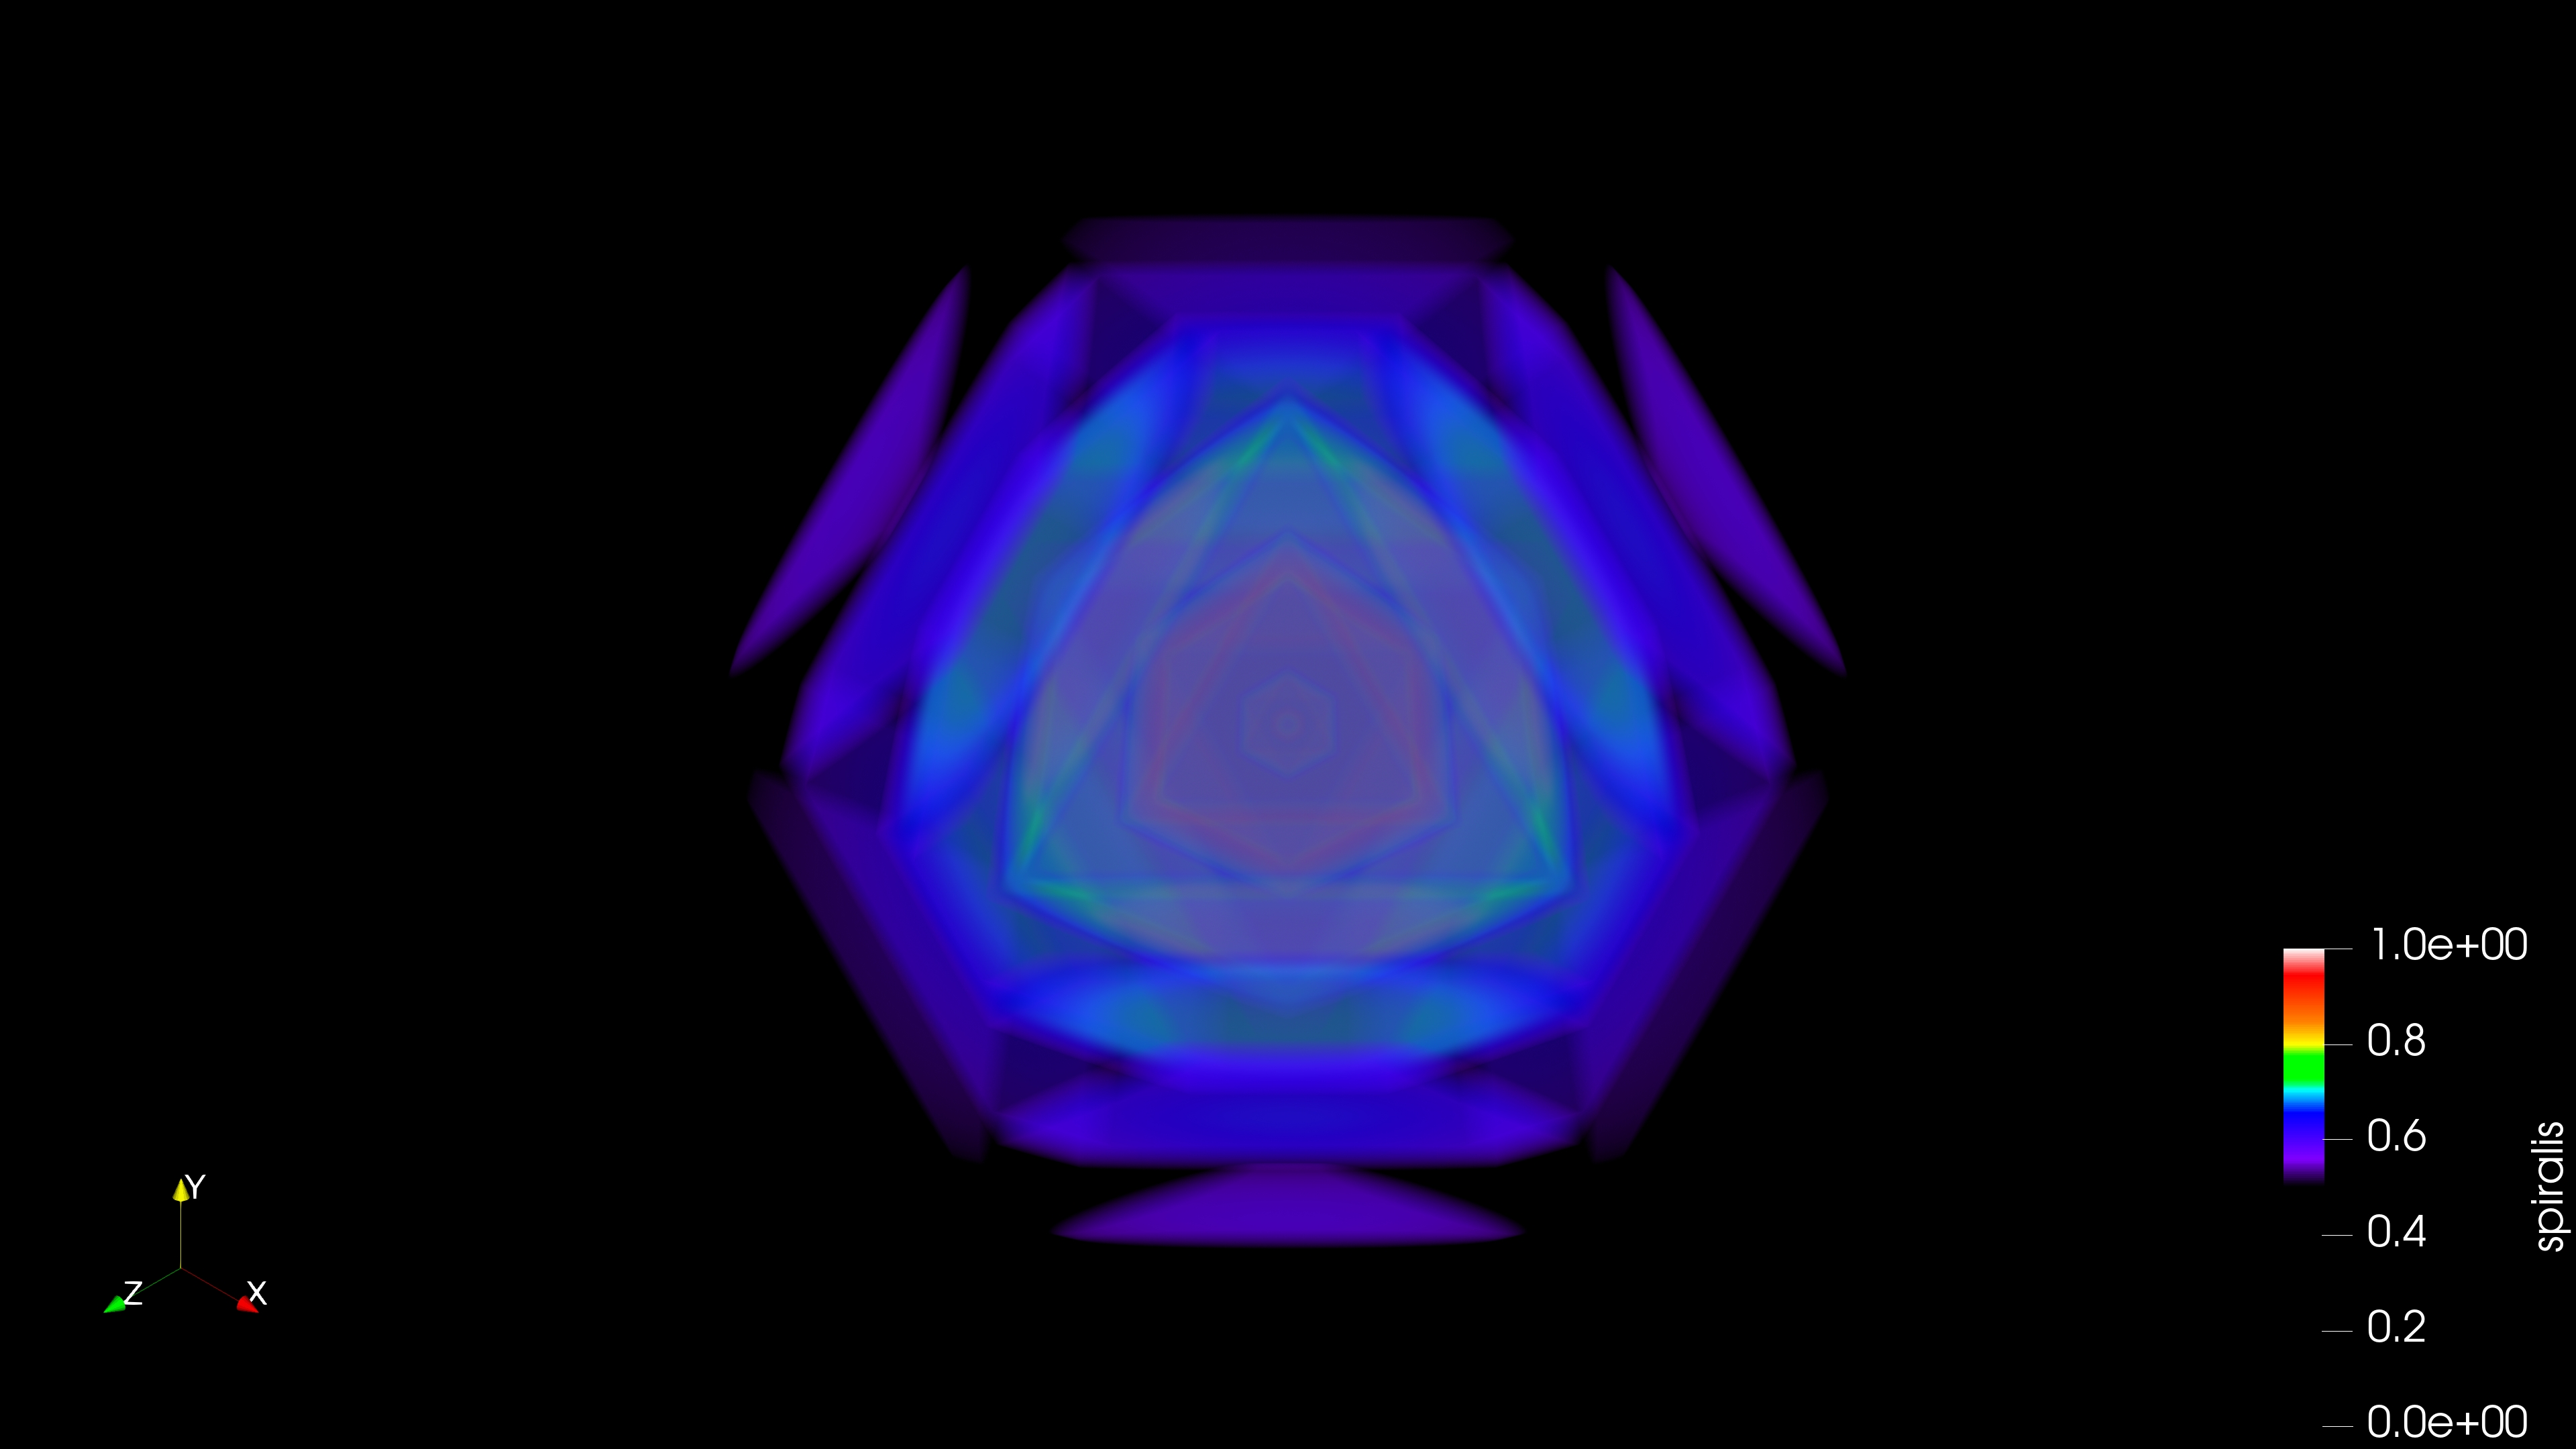
\includegraphics[width=0.85\textwidth]{Grafiken/05_Visualisierung/Proton/Proton_Volume_XYZ_Cam.jpeg}
  \caption{Darstellung der Proton.vti-Datei in Paraview}
  \label{fig:proton}
\end{figure}

Die erste stabile Spiralis-Struktur entsteht bei der achtfachen Raumüberlagerung. 
Sie bildet den energetischen Grundzustand des Feldes und markiert den ersten stationären Knoten der Raumenergie.
Das charakteristische Muster zeigt eine \emph{achtfache Symmetrie} um das Zentrum, die sich in allen höheren Strukturen wiederfindet. 
Die Visualisierung verdeutlicht die Stabilität dieser Anordnung — die Raumenergie faltet sich entlang der drei Raumachsen zu einem energetisch geschlossenen Knoten.
Der innere Bereich erscheint als konzentriertes, sphärisches Leuchten mit klarer Abgrenzung zum umgebenden Resonanzraum.
Das Proton stellt somit die elementare, selbststabilisierte Raumenergieeinheit dar.

\newpage

\subsection{Das Wasserstoffatom (H)}

\begin{figure}
  \centering
  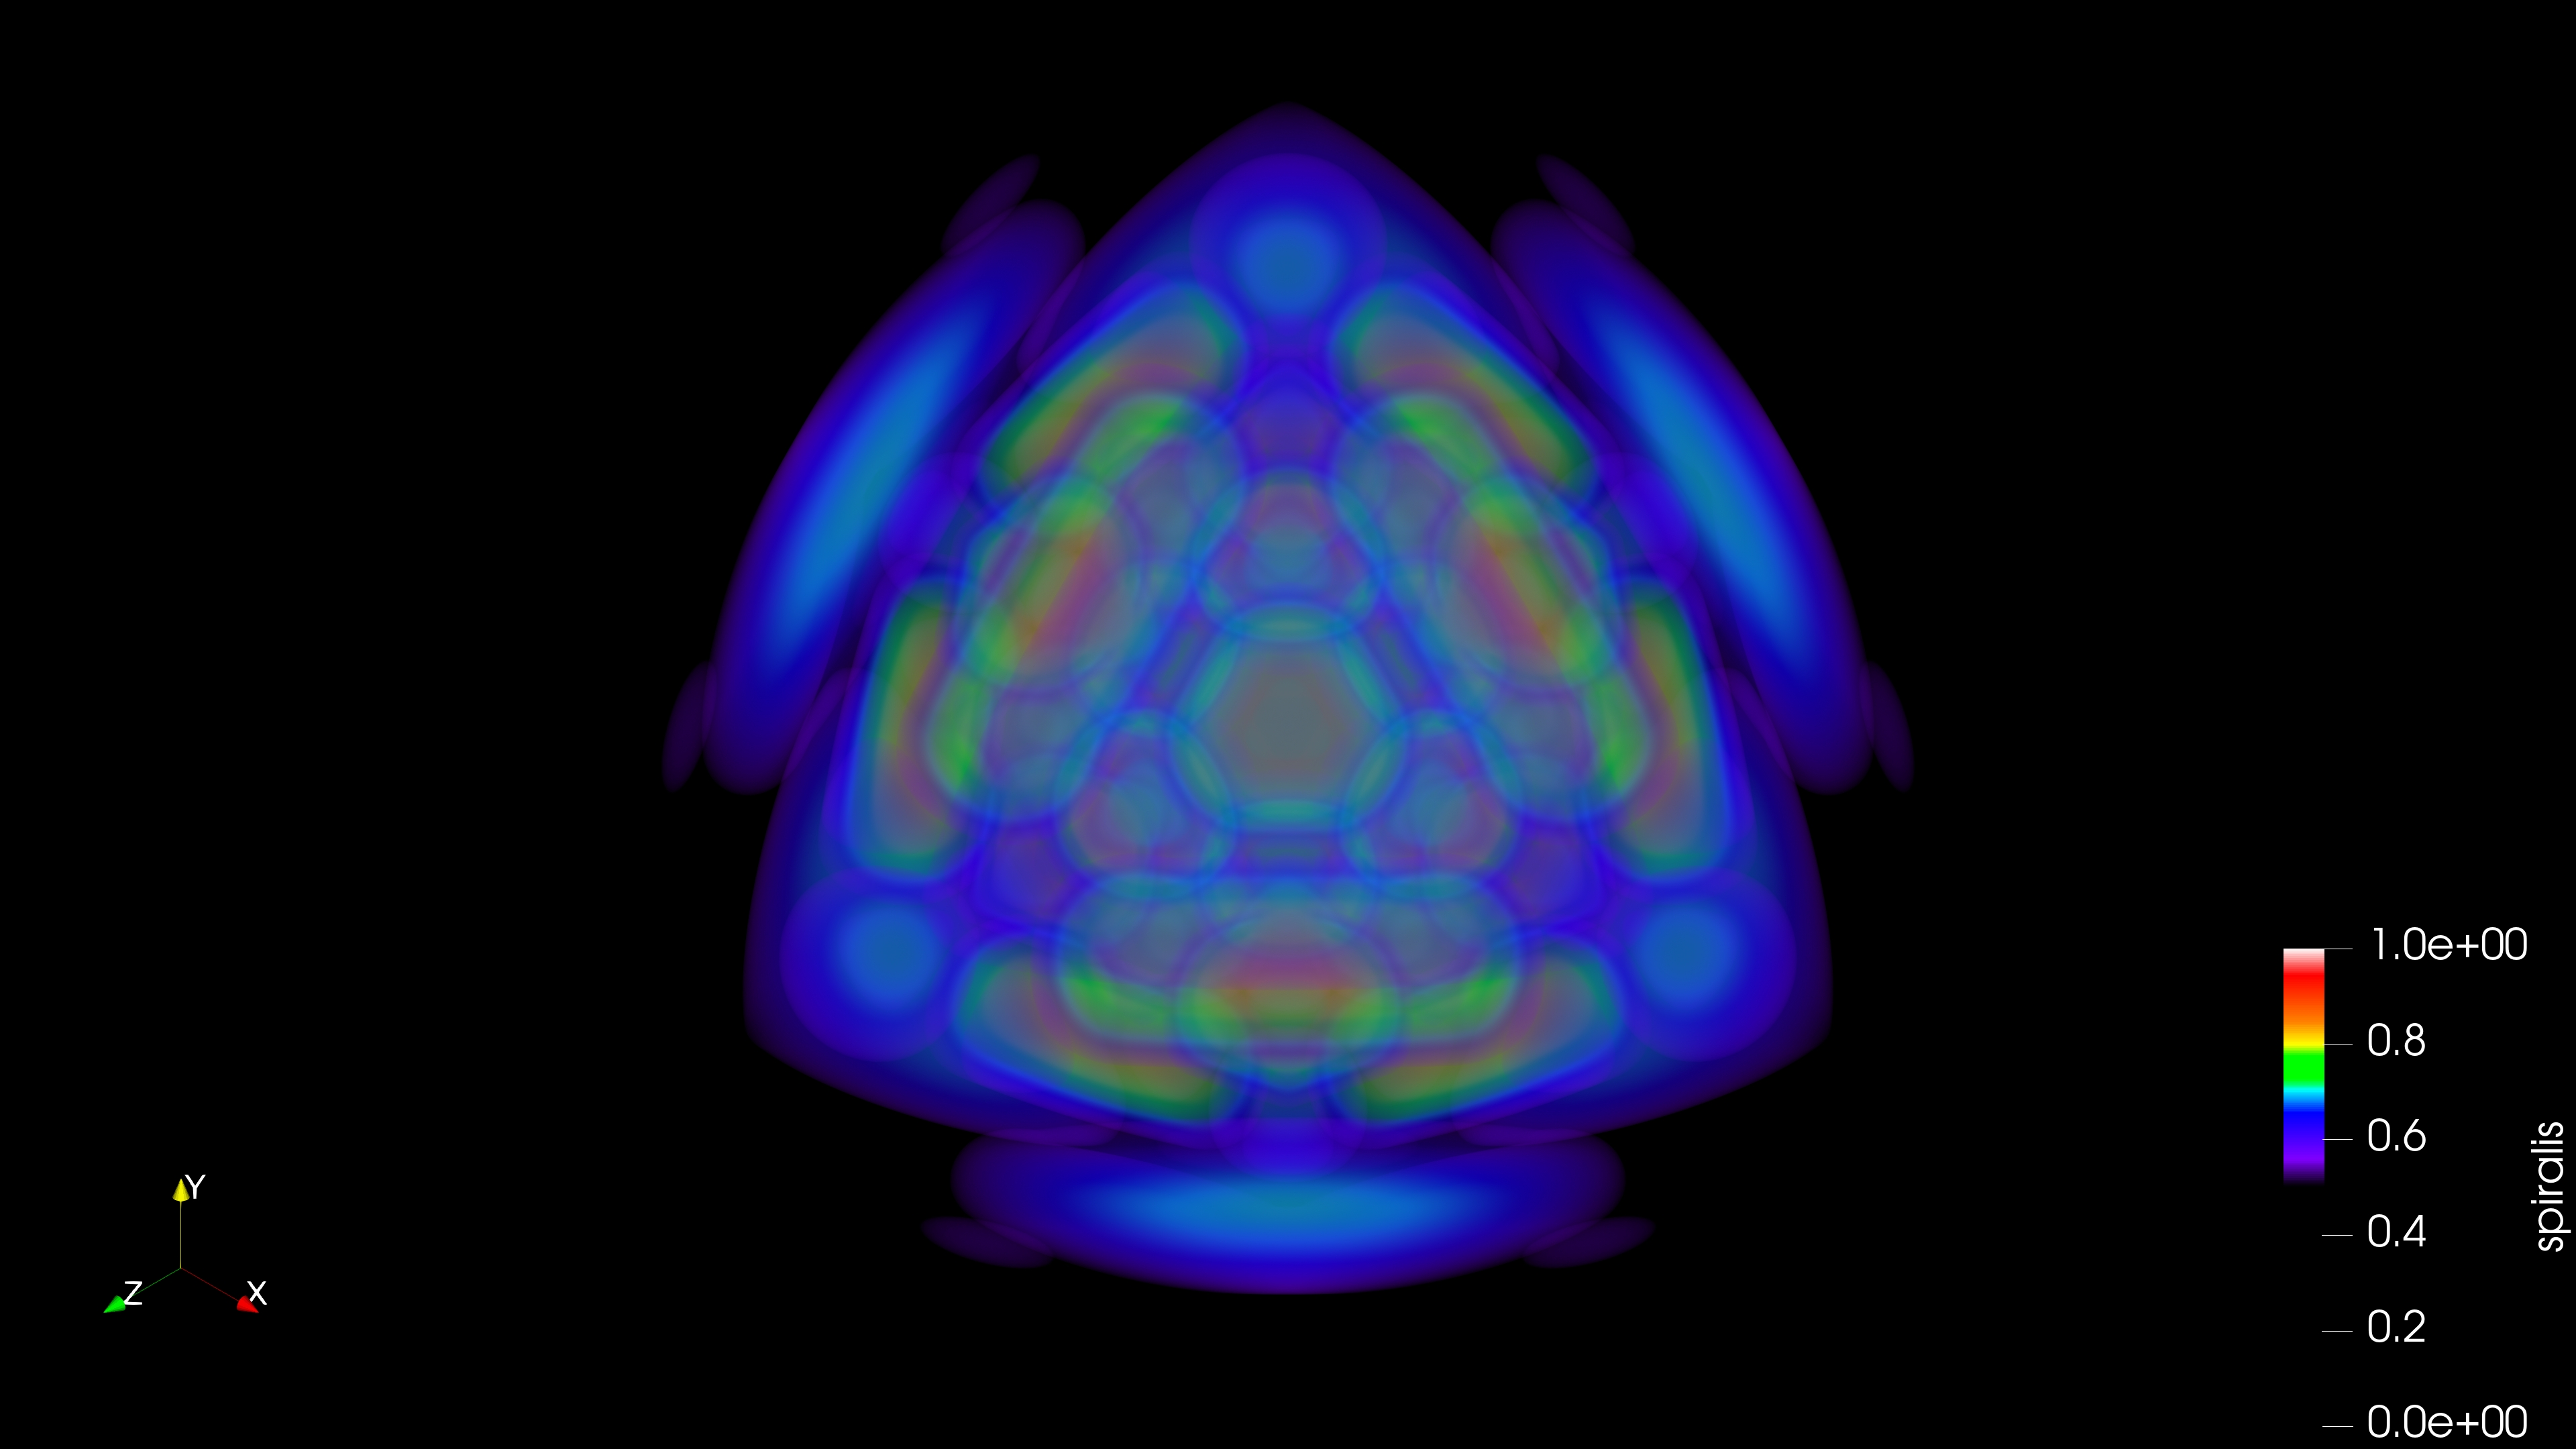
\includegraphics[width=0.85\textwidth]{Grafiken/05_Visualisierung/H/H_Volume_XYZ_Cam.jpeg}
  \caption{Darstellung der H.vti-Datei in Paraview}
  \label{fig:H}
\end{figure}

Durch achtfache Kopplung der Protonstruktur entsteht eine neue, räumlich erweiterte Energiedichteverteilung. 
Die Spiralis-Überlagerungen formen eine nahezu kugelsymmetrische Feldverteilung, deren Kern eine deutliche Steigerung der Energieintensität zeigt. 
Die Übergänge zwischen innerem und äußerem Feldbereich verlaufen harmonisch und erzeugen das typische visuelle Erscheinungsbild eines atomaren Energiepotentials.
Im Gegensatz zum Proton ist die Struktur hier bereits in der Lage, energetische Wechselwirkungen aufzunehmen, was sich in einer deutlichen Durchdringung des Raumfeldes zeigt.

\newpage

\subsection{Die Wasserstoffmolekülbindung (H2)}

\begin{figure}
  \centering
  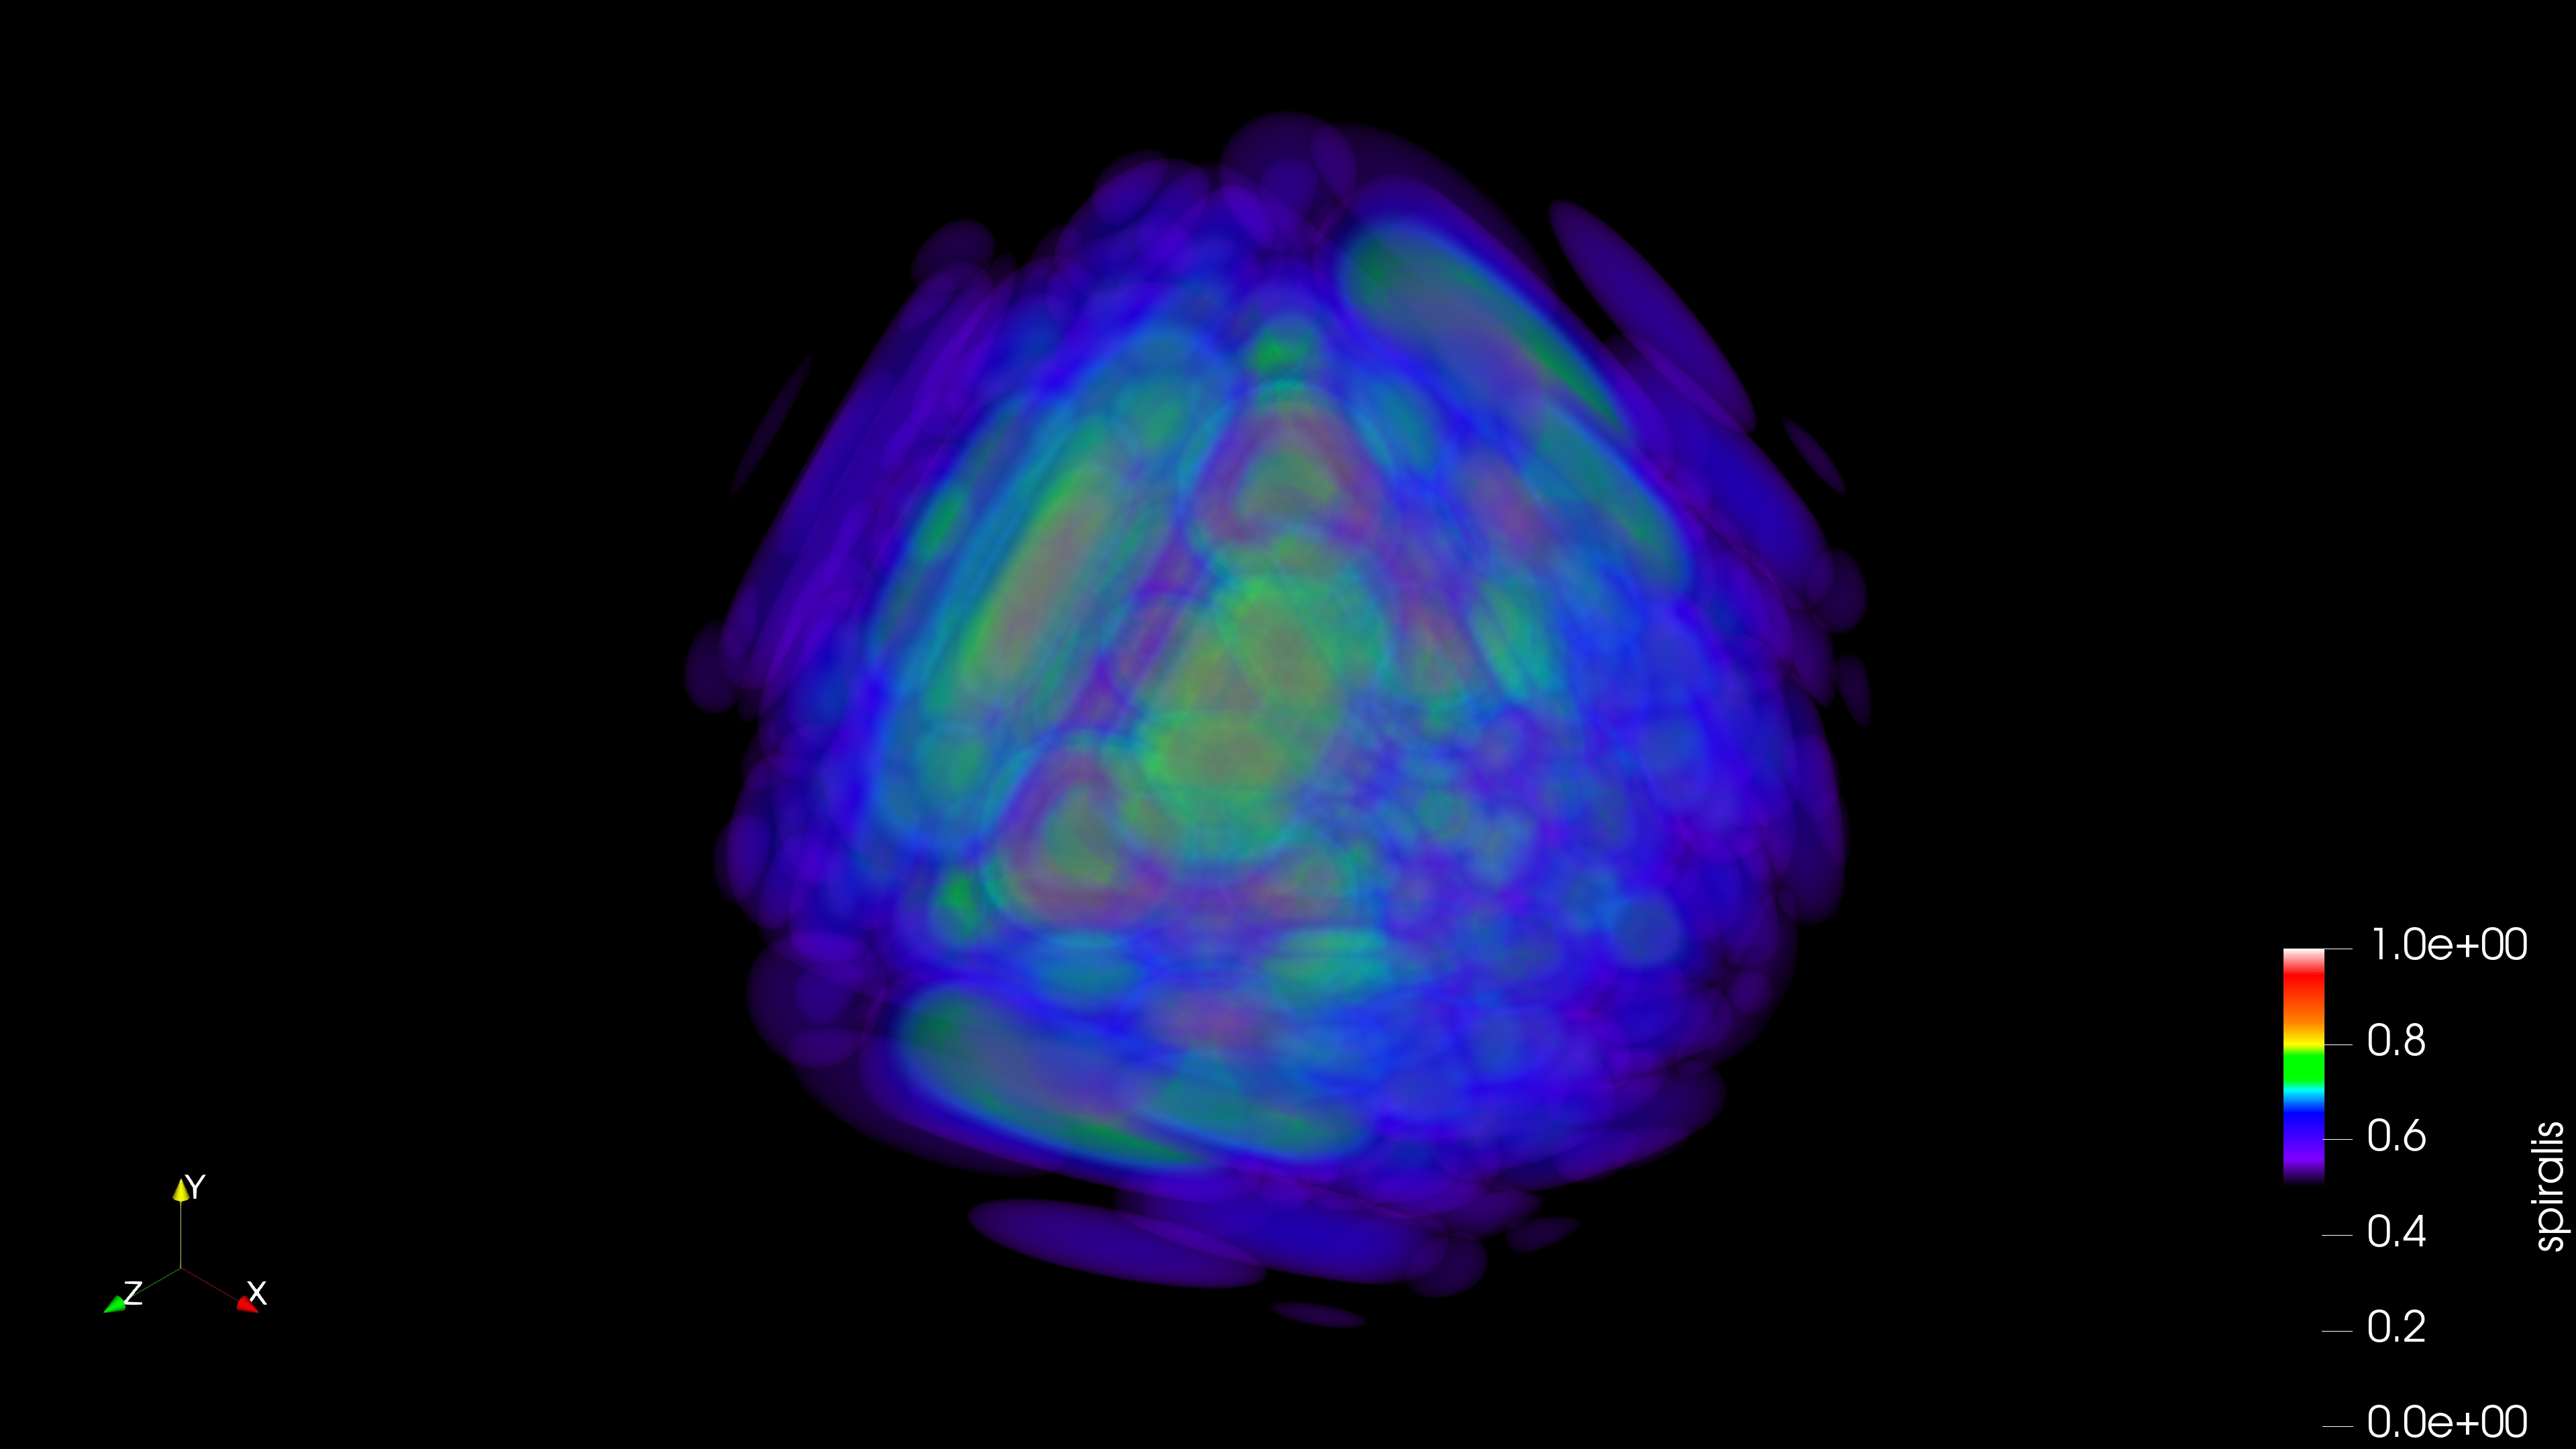
\includegraphics[width=0.85\textwidth]{Grafiken/05_Visualisierung/H2/H2_Volume_XYZ_Cam.jpeg}
  \caption{Darstellung der H2.vti-Datei in Paraview}
  \label{fig:H2}
\end{figure}

Die eindimensionale Kopplung zweier Wasserstofffelder erzeugt ein charakteristisches, länglich-symmetrisches Resonanzmuster entlang der Hauptachse. 
In der Visualisierung erscheinen zwei intensiv leuchtende Zentren, verbunden durch eine Region erhöhter Energiedichte — der molekulare Bindungsbereich. 
Diese Überlagerung stellt eine stabile, schwingungsfähige Konfiguration dar, deren Feldgeometrie die bekannten Eigenschaften einer kovalenten Bindung auf makroskopischer Ebene widerspiegelt. 
Die Raumenergie zwischen den beiden Zentren bleibt kohärent und weist auf eine periodische Kopplung der Feldknoten hin.

\newpage

\subsection{Das Sauerstoffatom (O)}

\begin{figure}
  \centering
  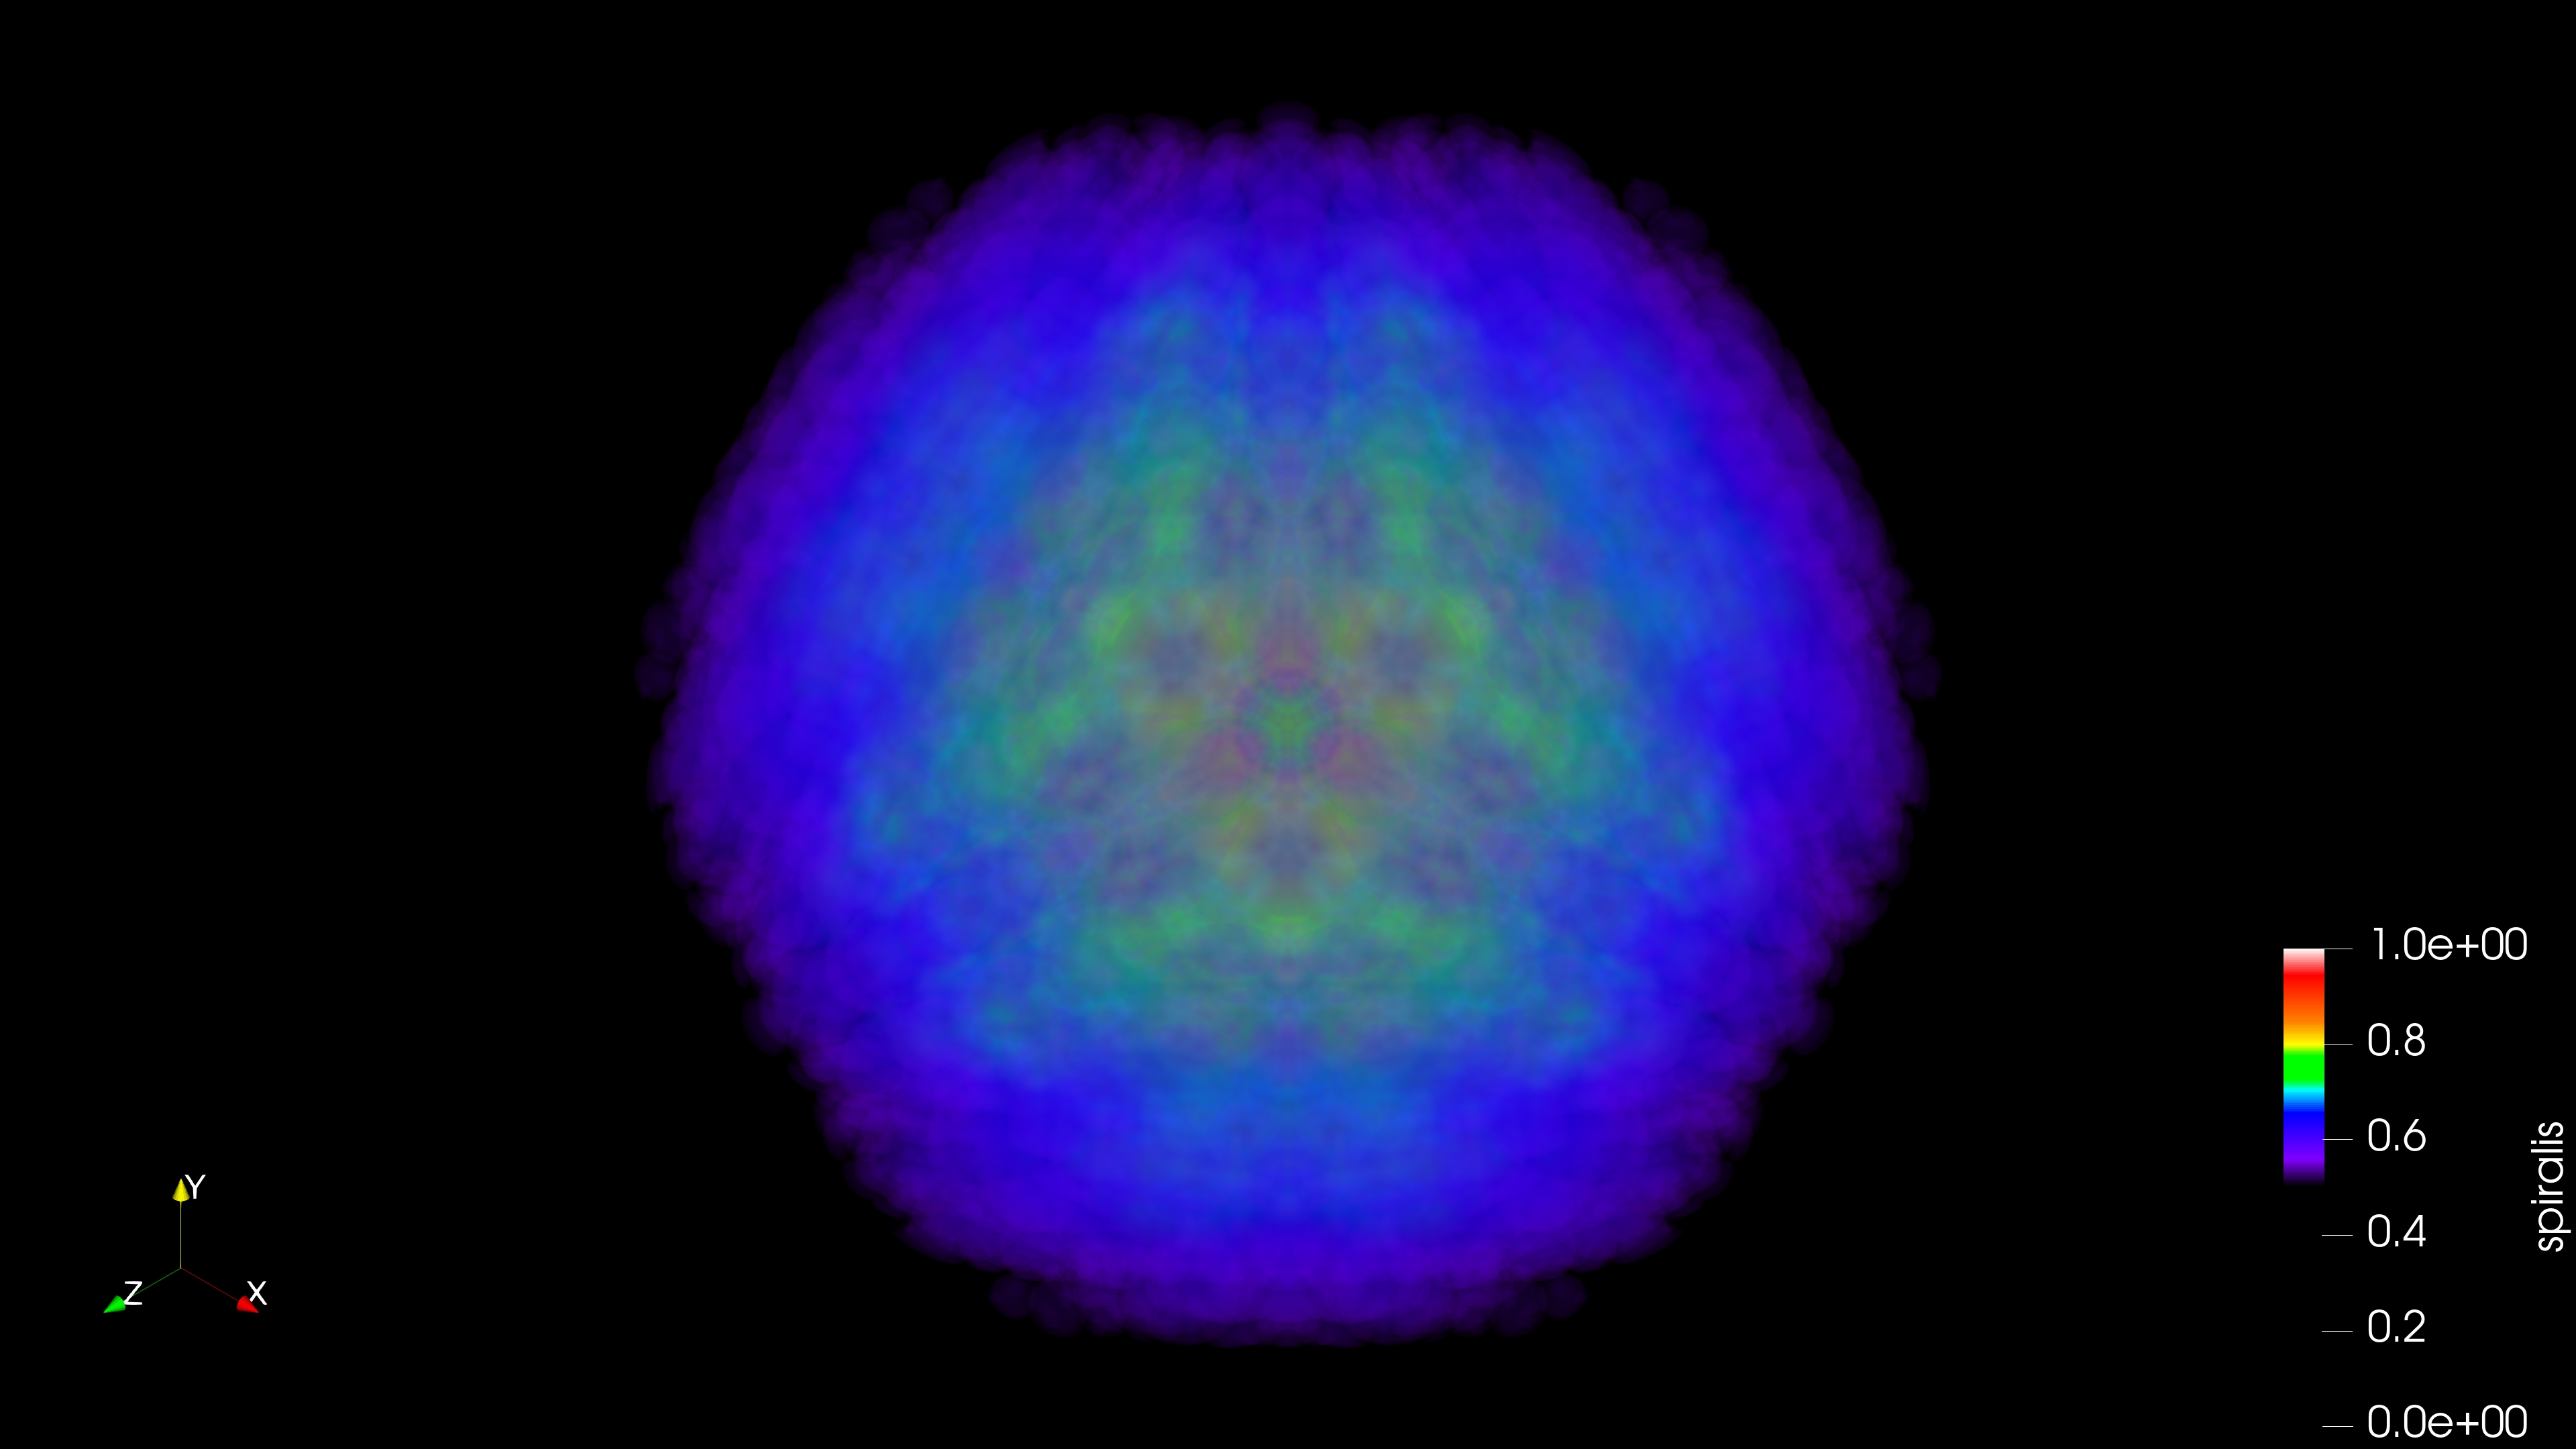
\includegraphics[width=0.85\textwidth]{Grafiken/05_Visualisierung/O/O_Volume_XYZ_Cam.jpeg}
  \caption{Darstellung der oxygen.vti-Datei in Paraview}
  \label{fig:O}
\end{figure}

Das Sauerstofffeld entsteht als nächsthöhere hierarchische Ordnung der Wasserstoffstruktur. 
Seine Spiralis-Verteilung zeigt eine erhöhte Komplexität der Knotenstruktur bei gleichzeitig stärkerer Verdichtung des Zentrums. 
Im Gegensatz zum Wasserstoff bildet das Sauerstofffeld ausgeprägte, mehrschichtige Resonanzhüllen, die auf eine höhere energetische Eigenstabilität hindeuten.
Die Visualisierung zeigt feine fraktale Muster, die in alle drei Dimensionen hineinreichen und die starke Bindungsfähigkeit dieses Elements auf energetischer Ebene erklären.

\newpage

\subsection{Das Diwasserstoffmonoxidmolekül (Wasser)}

\begin{figure}
  \centering
  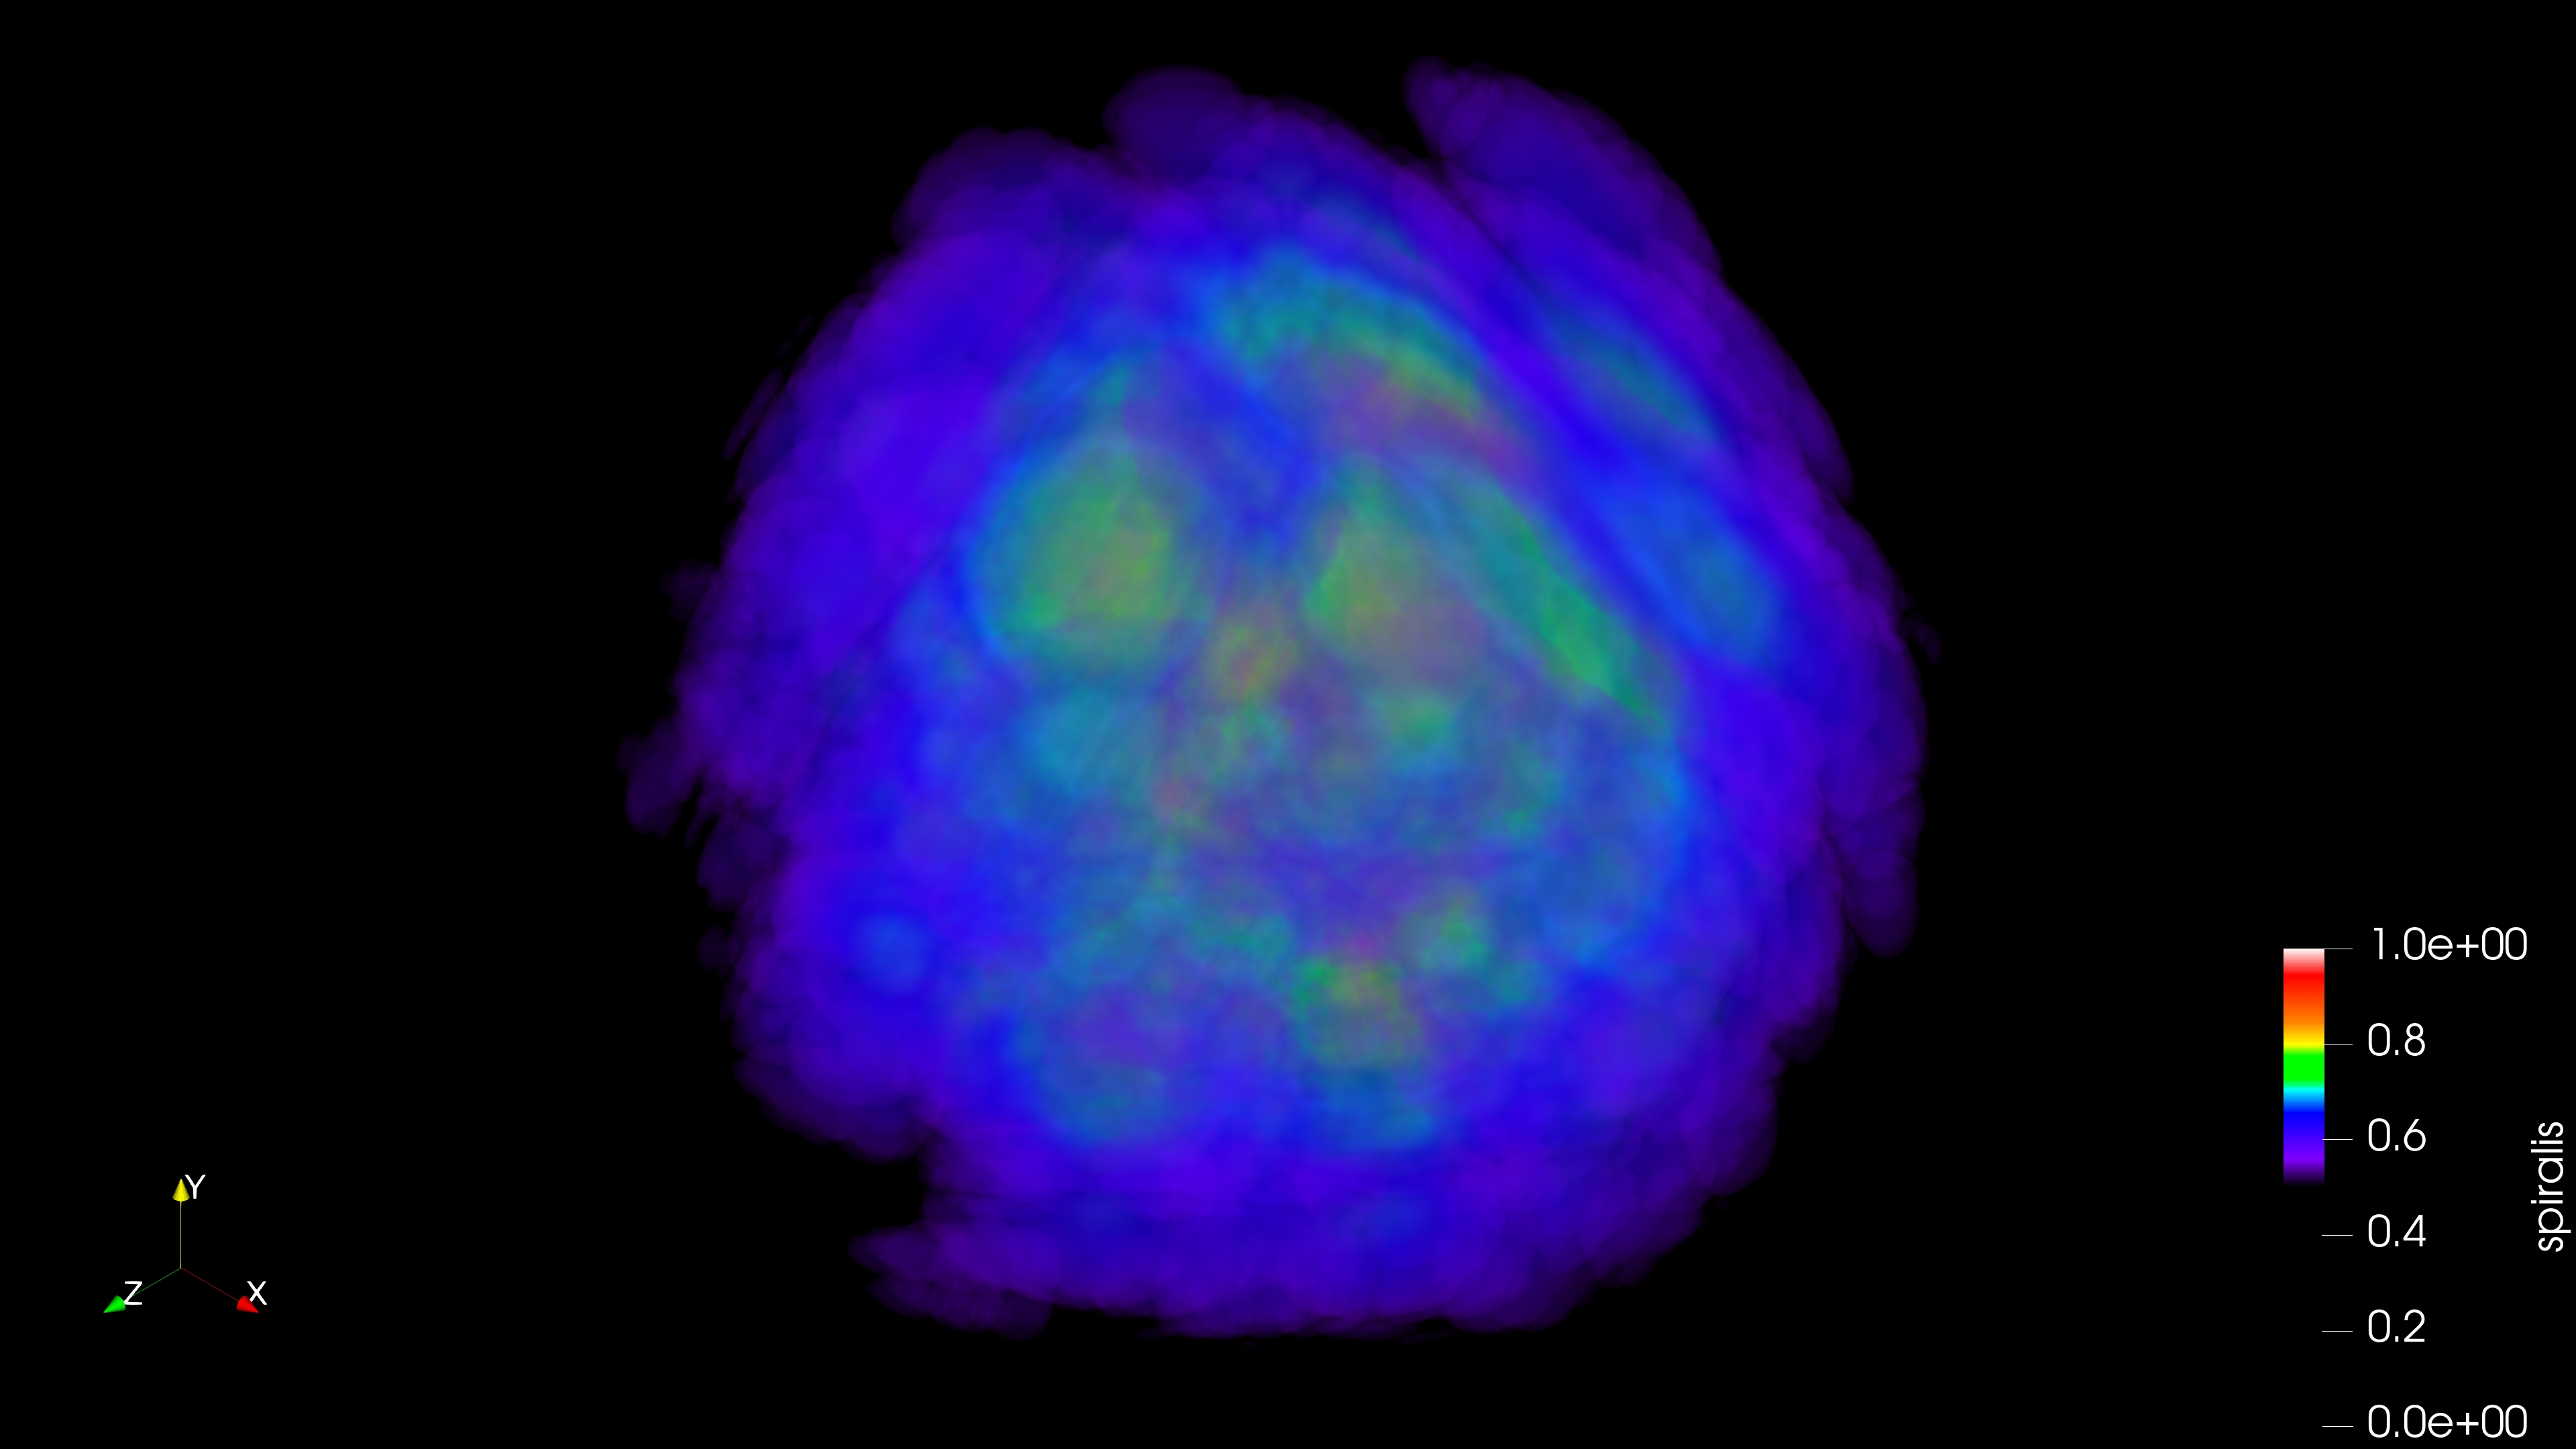
\includegraphics[width=0.85\textwidth]{Grafiken/05_Visualisierung/H2O/H20_Volume_XYZ_Cam.jpeg}
  \caption{Darstellung der H2O.vti-Datei in Paraview}
  \label{fig:H2O}
\end{figure}

Die dreidimensionale Kopplung von zwei Wasserstoff- und einem Sauerstofffeld führt zur komplexesten simulierten Struktur des Experiments.
Das resultierende Volumenfeld zeigt eine deutlich gerichtete Polarität, die sich als Asymmetrie in der Energiedichte manifestiert. 
Die beiden Wasserstofffelder koppeln in einem symmetrischen Winkel an das Sauerstofffeld, wodurch eine stabile Gesamtresonanz entsteht. 
Die Darstellung mit der \textit{EM-Colormap} offenbart farblich eine klare Polaritätsachse: energiereiche Bereiche (rot–gelb) im Zentrum und absorbierende Zonen (violett–blau) an den Polen.
Diese Struktur zeigt deutliche Übereinstimmungen mit den bekannten dipolaren Eigenschaften des Wassermoleküls. 
Sie demonstriert, dass die Spiralis-Funktion in der Lage ist, real beobachtbare Energieverteilungen geometrisch korrekt zu reproduzieren.

\vspace{0.5em}
\noindent 
Zusammenfassend zeigen die Ergebnisse, dass sich die gesamte beobachtbare Materie aus einer einheitlichen mathematischen Feldbeschreibung herleiten lässt. 
Mit zunehmender hierarchischer Ordnung steigt die energetische Komplexität, während das zugrundeliegende Muster der Spiralis unverändert bleibt.



\section{Schlussfolgerung}

Das numerische Visualisierungsexperiment zeigt,
dass die Spiralis-Funktion als reales Modell der Energieverteilung
im Raum fungieren kann.
Sie reproduziert aus rein mathemischen Vorgaben
beobachtbare Eigenschaften von Materie – etwa
stabile Symmetrieachsen, Energiepolarität und Absorptionseffekte.
Damit bestätigt das Experiment die in Kapitel~\ref{chap:mathematischer_rahmen_II}
entwickelte Annahme:
Die Spiralis-Funktion ist in der Lage, reales Energieverhalten
räumlich und zeitlich konsistent darzustellen.
